\chapter{Act I}



\begin{figure}
    \centering
    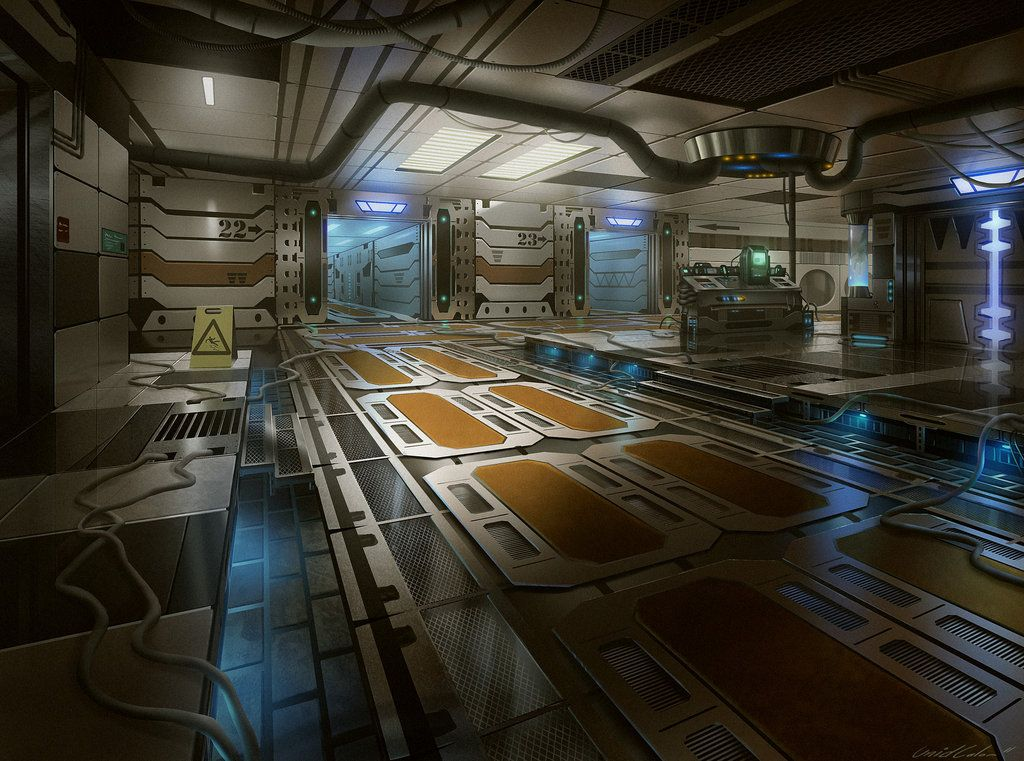
\includegraphics[width=.45\textwidth]{img/bg/interior.jpg}
\end{figure}



\begin{rpg-commentbox}{Chilling out}

    It is another day in the fire station. Paramedics are just tired of attending shift workers that overdose on never-sleeping pills. Firefighters are enjoying their meal and talking about whatever amenities they must talk about.

    \texttt{\textbf{MU/TH/UR:}} Let PCs have some time talking among themselves, play some rivalries and use NPC firefighters to guide the conversation if need be.
\end{rpg-commentbox}

\newsect

\begin{rpg-commentbox}{Fire alert}
    It would be yet another boring day for the majority of the crew when APOLLO puts the station on lock-down. There has been a huge fire and all non-essential personnel must remain on their quarters. Firefighters should proceed to San Cristobal Medical Facility immediately. 
    Traveling uses the Anchorpoint transit system. Each major section of the station has a firetruck and once out of rapid transit, firefighters can drive the truck through the station corridors. 

    \texttt{\textbf{MU/TH/UR:}} Use this time to roleplay the station chief. Debrief the situation, and what are the firefighters' priorities.
\end{rpg-commentbox}


\begin{rpg-commentbox}{Priorities}
    \begin{enumerate}
        \item Clear a path to the ambulance bay. Close hatches to suck all air of the bay, which is the primary source for the engulfing fire;
        \item Clear a path to the room (unknown designation) in between the staff quarters and environment control room. Secure any survivors in the room.
        \item Clear a path to the staff quarters where magnetic tapes and floppy data is kept. Save as much of the data as you can.
    \end{enumerate}
\end{rpg-commentbox}




\section{Special Rules}

\begin{rpg-commentbox}{Air supply}
    Players start with air tanks at full capacity (\texttt{\textbf{AIR 5}}). Roll for air whenever firefighters move into a new zone (other than the first). Roll for air after major checks, for example when a player rolls for \texttt{\textbf{HEAVY MACHINERY}} to open a hatch that is stuck or \texttt{\textbf{COMM TECH}} to override a control panel.

    Firefighters often carry an extra air tank if they know that the situation requires it. 
    There may be occasional supplies in strategic locations at the facility. It's up to the game \texttt{\textbf{MU/TH/UR}} to decide if players suffocate [for a bit] or if they can find them, but word of advice is that this will always keep players in their toes. 
\end{rpg-commentbox}  


\begin{rpg-commentbox}{Stress}
    When in duty, firefighters do not take any \texttt{\textbf{STRESS}} for eventual victims that they find. This may come as an aftershock.

    Firefighters often carry \texttt{\textbf{NAPROLEVE}} with them. They use the medicine to reduce their stress before it gets too critical, but due to regulations, a maximum of one dose is available to each player if the game \texttt{\textbf{MU/TH/UR}} decides so. Strongly recommended as this scenario barely has any places/moments where a player can reduce stress. 
\end{rpg-commentbox}   



\begin{rpg-commentbox}{Splitting the party}
    \texttt{\textbf{MU/TH/UR:}} Firefighters are in borrowed time. It's likely that they will have to split to cover all main objectives. Encourage that to the players and state that this is normal procedure. 

    It's not an alien game if everyone stays together watching each others back, right?
\end{rpg-commentbox}  

\begin{rpg-commentbox}{}
    \textbf{Act 1 ends when firefighters meet the Alien OR complete 2/3 of the objectives}
 \end{rpg-commentbox}

 \newsect


\section{Ambulance Bay}

\begin{rpg-commentbox}{The area}
    The ambulance bay is a small hangar with double-pressurized doors that allows landing of small shuttles. 
    It directly connects to the crisis stabilization center where any ICU patients are located. In the crisis stabilization area, there are 4 auto doc units and 2 auxiliary rooms for staff. A third 
    cylindrical room holds equipments and a small thermal battery can keep the area running even under the most dire situations.
    
    \texttt{\textbf{MU/TH/UR:}} One would have imagined that the patient brought by Weyland-Yutani would be here, but they are nowhere to be found.
\end{rpg-commentbox}  




\begin{rpg-commentbox}{Clearing a path}
    When firefighters get into the stabilization zone unit, the close the hatch behind them. There are three zones that they must  move through, each one representing one corridor after the initial corridor that marks the entrance.
    
    Due to the diamond shape format of the area, this 3 zones path is the same regardless if firefighters decide to take the right corridor or the left one.
    
    \texttt{\textbf{MU/TH/UR:}} Important details per zone/corridor:
    
    \texttt{\textbf{1st}} A firefighter that succeeds in a \texttt{\textbf{MOBILITY}} roll can safely reach the second corridor. Failure makes them fall, taking 1 point of damage, but still making the trip.

    \texttt{\textbf{2nd}} Once in 2nd corridor, a firefighter can cordinate with one that stayed at the entrance to use their tools to roll \texttt{\textbf{HEAVY MACHINERY}} (+2 if using a  \texttt{\textbf{halligan}}) to seal the 1st corridor and vent it, extinguishing any fire in the area. 

    While there is not as much fire here, visibility in this corridor is minimum and firefighters need to crouch and find their way to the next corridor. 
    \texttt{\textbf{MOBILITY}}, \texttt{\textbf{SURVIVAL}}, or \texttt{\textbf{SURVIVAL}} are options. Failure implies that a firefighter enters one of the ICU rooms losing precious time and forcing a roll on their air supply before they get to the final 3rd corridor.  

    \texttt{\textbf{3rd}} Once again, a \texttt{\textbf{HEAVY MACHINERY}} roll will make the previous corridor safe for passage for any other firefighters. When venting the second corridor, a patient that was in the floor suffocates. If you are comfortable, narrate their peril (see suffocating box).
    
    The fire here is extreme. The best option is to find hatches/panel of the fire supression system and try to manually trigger it filling the room with halon. 
    A \texttt{\textbf{COMM TECH}} roll can trigger the suppression mechanism.
    Contact of halon with some of the medical equipment in the area releases 
    noxious elements in the air. 
\end{rpg-commentbox}  


\begin{rpg-warnbox}{Suffocating}
    When the air is being venting out from the room a patient that was trapped starts to crawl towards one of the hatches. Firefighters see everything through the glass window. The patient grasps for air as the corridor eventually reaches zero-g and the body that was trapped calmly floats. Once the hatches are open, the body falls down and firefighters are reminded that ``\textit{in space no one can hear you screen}''.
\end{rpg-warnbox}
  

\newsect


\begin{rpg-commentbox}{Ambulance bay}
    Most of the structure is compromised here. Firefighters need to reach the hangar doors panel and initiate the standard landing procedures what will open the shuttle door and eventually leave the bay in vacuum. 

    The panel is too damaged for a \texttt{\textbf{COMM TECH}}, so firefighters need to do it manually. Pumping the lever does require  physical effort and the lever needs to be pushed thrice before it starts the standard landing procedures. 

    \texttt{\textbf{MU/TH/UR:}} Players can rotate who pushes the pump, but anyone who does it must immediately roll for \texttt{\textbf{AIR}}. If a single player does it, that means 3 consecutive rools.
\end{rpg-commentbox}  

\newsect


\begin{rpg-commentbox}{Conclusion}
    Only smoke remains in the area, but most of the fire has been dealt with. Multiple bodies can be found through the corridors, but they are the expected casualties.
    
    \texttt{\textbf{MU/TH/UR:}} The fire chief communicates with the firefighters in the area commending them for their job  and ordering them to proceed either to the mysterious room zone or the data drive area. 

    The chief's appraisal reassures the firefighters, relieve \texttt{\textbf{1 STRESS}} from any players who where in the area.
\end{rpg-commentbox}  



\clearpage

\section{Mysterious Room}

\begin{rpg-commentbox}{The area}
    This room is located close to the sedation ward and near the entrance of the staff quarters where data drivers are located. It is bigger than any ICU in the crisis stabilization center and it is in fact the most well equipped ICU in the facility.

    It's purpose is to house any VIP with medical issues in a secure location away from any curious eyes. The \texttt{\textbf{VIP ICU}} also has equipment for biopsies and containment of any foreign substance or parasite that might be found. 

    This is particularly important in case of viruses, as companies, such as Lasalle Bionational, are always in the look for new chemical compounds or elements that can be bio-engineered and turned into assets.

    The fire has not spread to this area yet. The two nearby areas, environment control and the sedation ward have fires. A skilled firefighter will notice that fire in these areas is not expected if the source of fire is in the ambulance bay.

    \texttt{\textbf{MU/TH/UR:}} One unfortunate person lies dead in an auto doc pod.
    It's clearly visible that they were restrained and their stomach is open. Even the firefighters take a \texttt{\textbf{STRESS}} point.

    There is liquid dripping from one of the biopsy pods that is shattered. Further inspection shows one medic or scientist dead. After the appropriate check a firefighter can uncover that the medic had their ankle cut open and thus, they bleed to death. 
\end{rpg-commentbox}   



\section{Data Drives}

\begin{rpg-commentbox}{The area}
    This area is where the facility personnel rest and relax whenever they are not in a shift. There is a kitchen, cabinets, chemical showers, and bunk beds in the area. 
    
    The far north-east corner of the area also has the computational grid and data drives of the facility. One would expect a dedicated room or area for that but it seems that the staff quarters were actually pushed to the server room as the facility grew in size. 

    A few staff members are in the area, including a comm expert that is frenetically going over the data grids as two Weyland-Yutani mercenaries watch him. 

    \texttt{\textbf{MU/TH/UR:}} The entrance door is barred. \texttt{\textbf{HEAVY MACHINERY}} or \texttt{\textbf{COMM TECH}} can force it open. 
\end{rpg-commentbox}  



\section{End of Act}



